\section{System Architecture: Adapted version of the “Inner Thoughts” framework}

% ---------------------------------------------------------------------------------------------------------------------
\subsection{Overview}
\label{sec:adapted-inner-thoughts}

\begin{figure}[H]
  \centering
  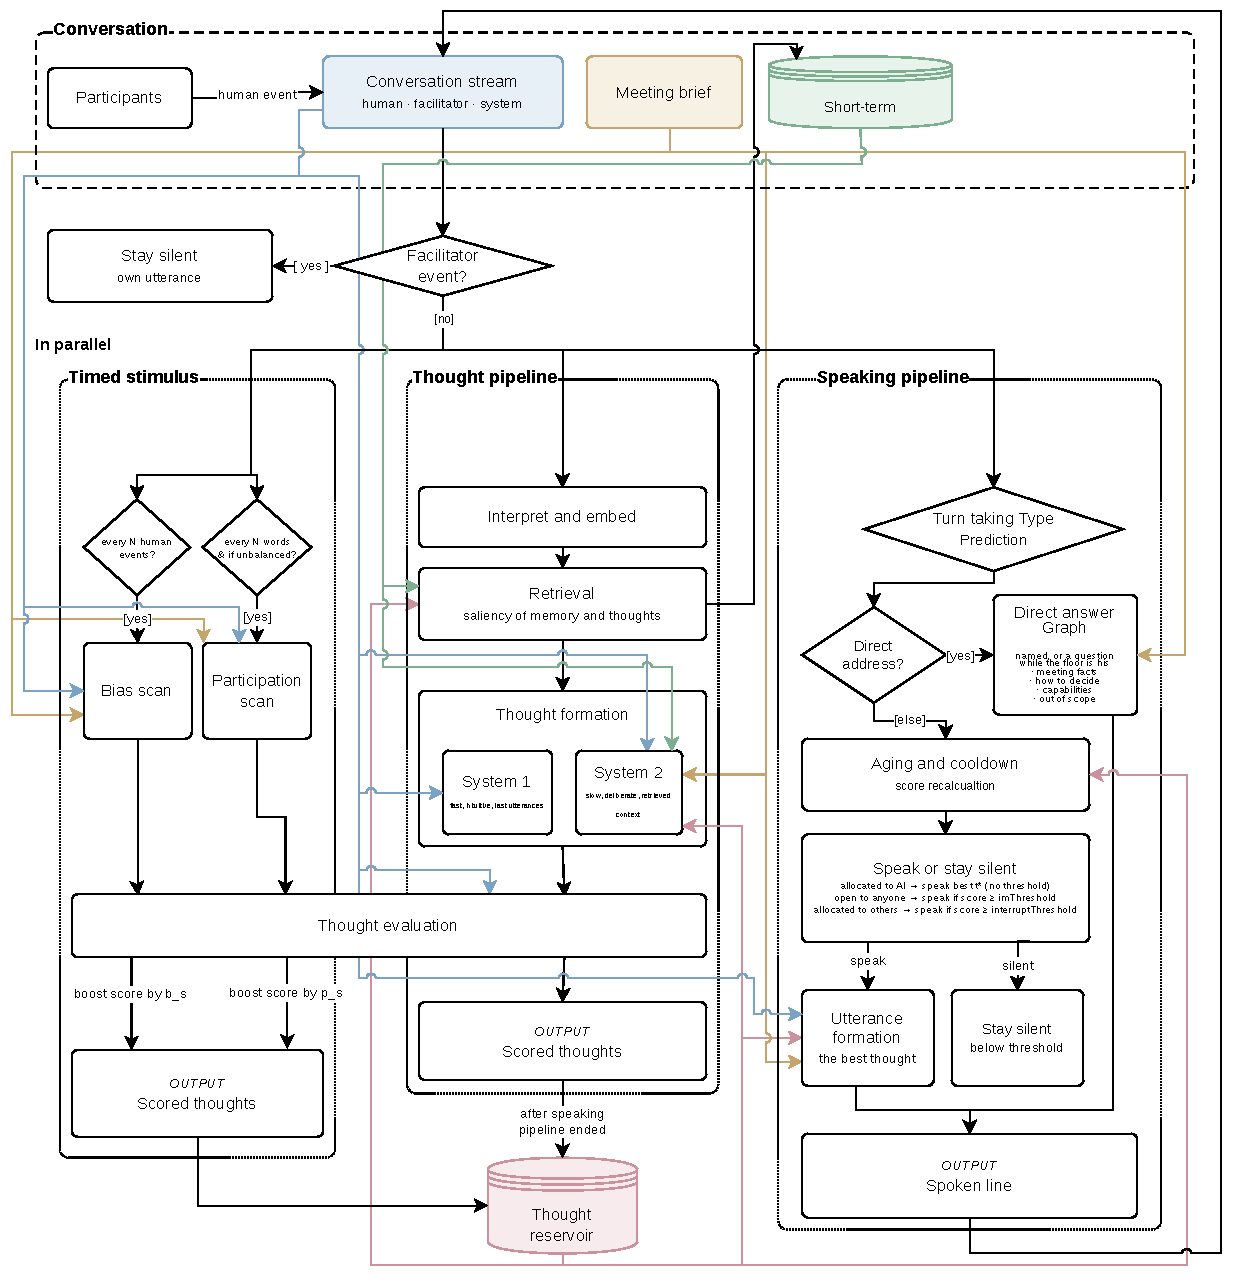
\includegraphics[width=0.99\textwidth]{assets/figures/04/system-architecture.pdf}
  \caption{System Architecture: Adapted version of the “Inner Thoughts” framework
    \figsource{Own illustration based on "Inner Thoughts" by Liu et
  al.\cite{liuProactiveConversationalAgents2025}, created with draw.io.}}
  \label{fig:system-architecture}
\end{figure}

\begin{figure}[H]
  \centering
  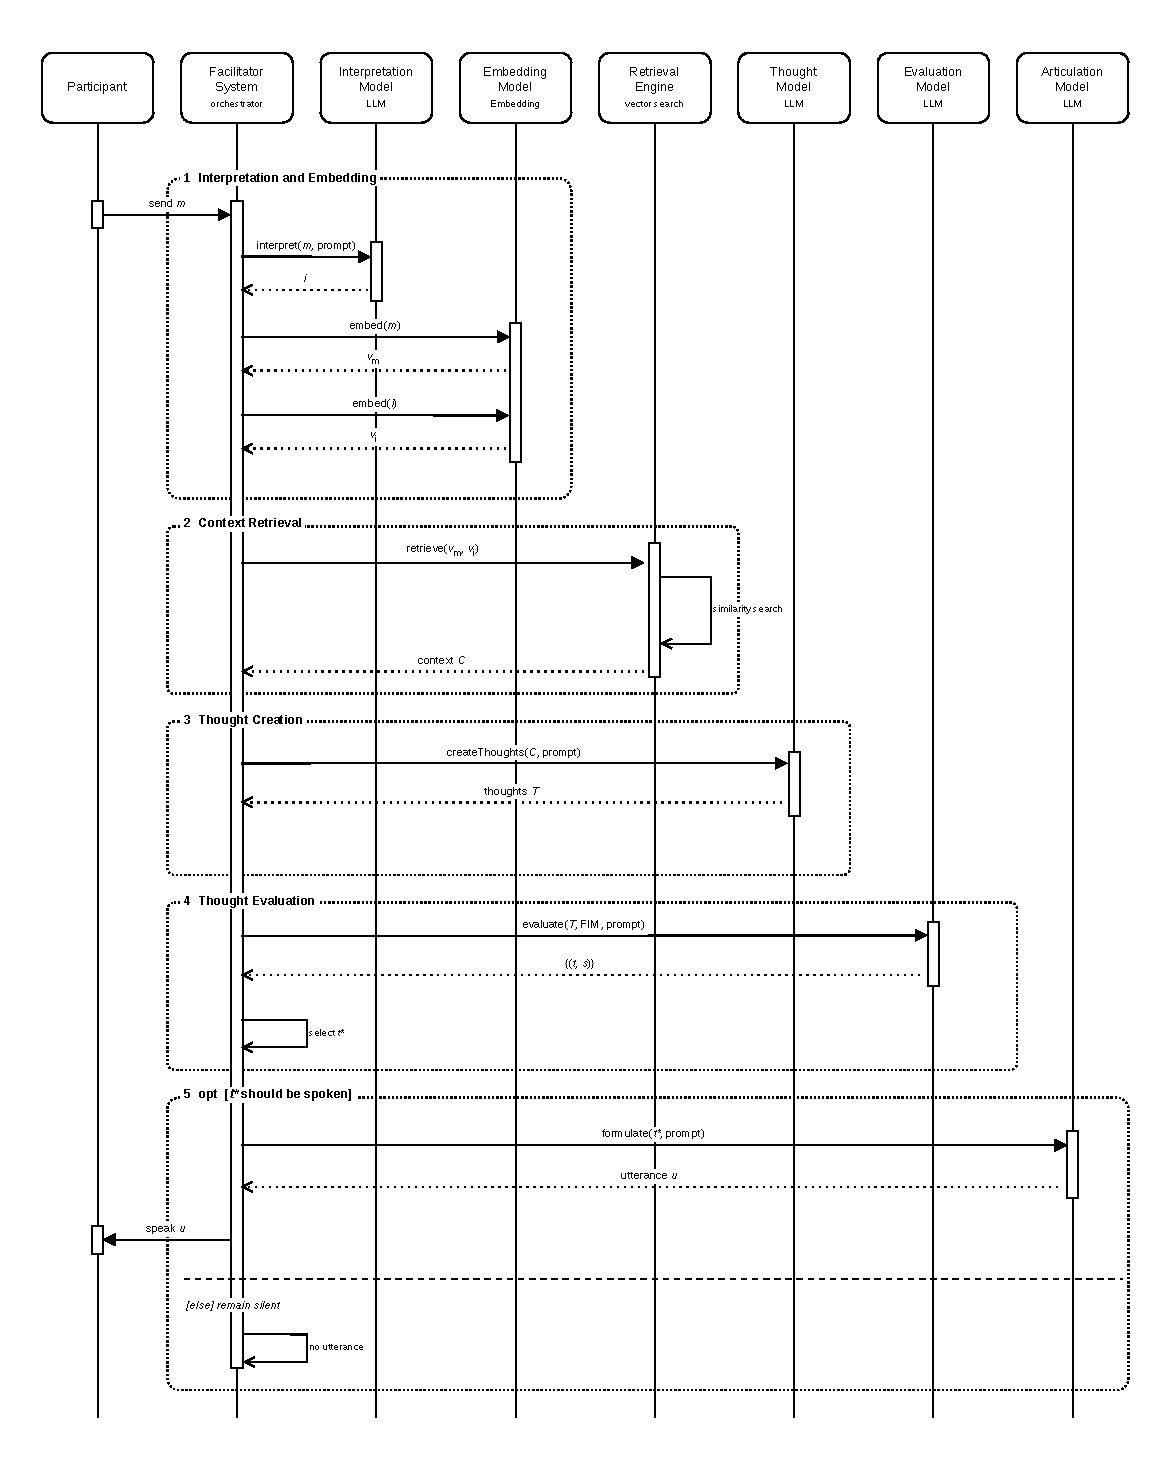
\includegraphics[width=0.97\textwidth]{assets/figures/04/thought-pipeline-sequence.pdf}
  \caption{Thought Pipeline Sequence: Sequence of the thought pipeline
    \figsource{Own illustration based on "Inner Thoughts" by Liu et
  al.\cite{liuProactiveConversationalAgents2025}, created with draw.io.}}
  \label{fig:thought-pipeline-sequence}
\end{figure}

Das System ist stark abgeleitet von dem inner thougs frame work. Grundlegende kontxepte wie die thoug
generiung, evalutung und die trun taking prediction wurden übernommen, aber an diesen user case und
insbesondere an das live szenario angepasst.

Das Inner Thoughts- Freamwork von Liu et al. ist in deren version eher für interaktionen ausgelegt die als
soziales Plaudern kotegorisertet werden können. Dies ist nicht was ein Faciliator machen würde. Die Idee ein
KI-System anhand einer intrsisichen motivation zu modellieren, bevor jemand etwas zu einer Gruppen discussion
beiträgt, ist dennoch auch für diese ARbeit relevant.
Insbesondere weil dieser Ansatz darauf hindeutet eine erhöhte Genauigkeit bei self-trun-allocation zu erzeugen.

Die Autoren wiesen in der Diskussion der Arbeit \cite["8.2 Apllying Inner Thougs Beyond Casual
Conversations"]{liuProactiveConversationalAgents2025} selbst darauf hin, dass sich das System durch anpassungen der
Bewertungskriterien auf aufgabenorietnerte Kontexte anpassen lässt und zielorientiertes praktives Handeln
ermöglichen kann. Sie schalgen vor für weitere arbieten das system mit domain-specifische heuristiken
anzupassen, um die interaktionen an real-world tasks zu orientieren. Aus diesem Grund wurdne prozessuale
ideen aus dem ursprungs modell größten teils übernommen und die entsprechendne promts angepasst.

Das system reagiert auf eingehende Gesprächsereignisse. Ereignisse sind menschliche Äußerungen und
Facilitator-Äußerungen. Bei jedem Ereignis, das nicht die eigene Äußerung des
AI-Systems ist, laufen drei Pipelines gleichzeitig und teilen sich vier Speicher: den Gesprächsstrom, den
Meeting-Brief, das Gedächtnis und das Gedankenreservoir.

**Zeitgesteuerter Stimulus** (Timed stimulus) ist eine langsame Prüfung. Nach einem Zeitplan, und nur wenn
sein Gate öffnet, liest er das gesamte Transkript und fügt einen Prozessgedanken hinzu: entweder eine Prüfung
auf Bias und Einseitigkeit oder eine Prüfung der Redeanteile. Seine Aufgabe ist, Risiken sichtbar zu machen,
die Reaktionen von Zug zu Zug verpassen.

**Gedankenpipeline** (Thought pipeline) ist fortlaufende verdeckte Kognition. Sie deutet das aktuelle
Ereignis, aktualisiert, welche Erinnerungen und früheren Gedanken salient sind, bildet neue Gedanken und
bewertet, wie stark jeder eine Intervention rechtfertigt. Ihre Aufgabe ist, ein Reservoir von
Facilitationsimpulsen bereitzuhalten, bevor eine Sprechgelegenheit entsteht.

**Sprechpipeline** (Speaking pipeline) ist die Entscheidung, das Wort zu ergreifen. Sie klassifiziert, wem
der nächste Turn gehört, beantwortet eine direkte Frage aus dem Meeting-Brief, wenn die Äußerung an den
Facilitator gerichtet ist, und spricht andernfalls den stärksten bereits im Reservoir liegenden Gedanken oder
bleibt stumm. Ihre Aufgabe ist, nur dann einzugreifen, wenn Rederecht und Bewertung des Gedankens es rechtfertigen.

**Gesprächsstrom** (Conversation stream). Ein geordnetes Protokoll aus den live während des meetings
transkirbierten sprachbeiträgen der meeting teilnehmden so wie der KI-System.

Jedes Ereignis wird seriell verarbeitet.

Hat gerade das KI-System selbs einen Beitrag zur conversation beigetragen, so wird diese nicht erneute
verarbeite, weil das system sonst auf seine eignee Beträge reagieren könnte.

Jedes andere Ereignis startet alle drei Pipelines. Die beiden Scans haben zusätzliche Gates und tragen sonst
nichts bei.

% ---------------------------------------------------------------------------------------------------------------------
\subsection{Though Pipeline}

\textbf{Interpret and embed}
Bei einem menschlichen Ereignis wartet die Pipeline, bis Deutung und beide Embeddings gespeichert sind. Die
Deutung ist eine Lesart der Äußerung in ein bis zwei Sätzen vor dem Hintergrund des jüngsten Transkripts.
Embeddings verwenden dasselbe Embedding-Modell wie Erinnerungen und Gedanken.

\textbf{Retrieval}
Die Salienz von Langzeitgedächtnis, Kurzzeitgedächtnis und bestehenden Gedanken wird gegen das aktuelle
Ereignis neu berechnet. Anschließend wird das Ereignis an das Kurzzeitgedächtnis angehängt.

\textbf{Thought formation}

Im ursprünglichen Modell von Liu et al. werden generierte Gedanken primär danach bewertet, wie stark sie die
"persönliche Relevanz" die individuellen Interessen oder die einzigartigen persönlichen Kenntnisse des
Agenten widerspiegeln (TODO: prüfen bzw. konkretisieren wie die heuristik tatsächlich ist). Dies mag für
generische Conversationen geeigent sein, da dieser Ansatz Authentizität und
Sympathie in infromellen, sozialen Unterhaltungen erhöht, ist für einen AI-Moderator in zielorientierne
Meetings die durch Hidden Profile geprägt sind, allerdings ungeeiengt. Wenn die Gedanken des AI-Moderator
primär danach bewertet würden, wie stark sie seinen "persönlichen Interssen" wiederspieglen, verfällt er in
dassaelber fehlerhafte Verahltensmuster, das zu verzeruung in hidden profile situationen führen kann. Er
bringt eingen Meinungen oder Präferzene ein statt die diskussion neutral zu strukturieren. Strukturelle
prozeduelle Gedanken würde in der aktuellen Heurisik voraussichtlich mit zu niederiger Relevanz bewertet werden.

Bei der Anpassung der Heurisitken und prompts wurden sowohl die Literatur als auch die erkentnisse aus den
Interviews berücksichtigt. Die Evaluierungs-Heursitik zu bewertung der Gedanken wurde so angepasst, dass sie
das kognitionspyschologsche Fundament des Innter Thoughts-Modelles (basierend  auf grice, Sacks, Goffman und
Berly) mit en organisationspsychologischen Prinzipien zur Kompenstation des Shared Information bias (Stasser \&
Titus; Brodbeck et al.) und den HCI-Richtlinen für inklusive Moderation (Houttie et al; Davison) kombiniert.

System 1 und System 2 laufen gemeinsam.

**System 1** ist eine schnelle Prozessreaktion auf die letzten fünf Ereignisse: Anerkennung, Tempo, eine
leichte Einbezugskontrolle oder Zurückhaltung. Es liest nur dieses Transkript. Seine Stimuli sind diese fünf
Ereignisse. Der Gedanke hat unter 15 Wörter.

**System 2** ist überlegt. Die Standardanforderung sind zwei Gedanken. Der Prompt enthält die letzten
fünfzehn Ereignisse, den Meeting-Brief, bis zu fünf saliente Langzeiterinnerungen, bis zu fünf saliente
Kurzzeiterinnerungen und bis zu drei saliente frühere System-2-Gedanken. Jeder Gedanke zitiert eines oder
mehrere dieser Elemente. Ein Slot für eine Verfahrensrichtlinie ist vorhanden und derzeit auf die Aussage
festgelegt, dass keine Richtlinie aktiv ist. Gedanken haben unter 15 Wörter.

\textbf{Thought evaluation}

Jeder neue Gedanke wird von 1 bis 5 als intrinsische Facilitationsmotivation bewertet: wie stark ein
neutraler Facilitator ohne Entscheidungsbefugnis ihn jetzt äußern wollen würde. Der Bewerter sieht die
letzten fünfzehn Ereignisse und bis zu zehn saliente Langzeiterinnerungen. Die Bewertung wird anschließend
mit \(1{,}01\) hoch der Anzahl der Turns seit der letzten Äußerung des Facilitators multipliziert und auf das
Intervall von 1 bis 5 begrenzt. Dieser Wert wird als Basisbewertung \(s_0\) zusammen mit dem
Bewertungszeitpunkt gespeichert. Eine fehlgeschlagene Bewertung speichert die Basisbewertung 0 und schließt
den Gedanken damit von der späteren Auswahl aus.

Auch hier wurde die Heuritiken also der zu grunde liegen Promt angepasst. es wrude isch an der urspürnglichen
promt stuktur oritentiert und dieser [TODO]

% ---------------------------------------------------------------------------------------------------------------------
\subsection{Speaking pipeline}

\textbf{Turn-Taking-Prediction}

Ein Klassifikator liest die letzten fünf Ereignisse und weist das nächste Rederecht zu:

- **facilitator** — der jüngste Turn richtet sich an den Facilitator, oder er ist eine Frage zu Prozess,
Struktur oder weiterem Vorgehen;
- **group** — ein gelisteter Mensch wird genannt, der jüngste Turn ist eine Domänenfrage, oder nur die
Menschen können den Gegenstand weiterführen;
- **anyone** — das Rederecht ist offen.

Diese Idee udn grun strukur ist ebenfalls aus dem Inner Thoughts Framework übernommen der Prompt zu turn
taking prediction wurde auf die situation des Faciliator gesehen angepasst.

\textbf{Direct answer graph}

Bevor ein Gedanke aus dem Reservoir gewählt wird, prüft das System, ob jemand den Facilitator um eine
Auskunft bittet. Eine Auskunft wird sofort beantwortet. Alles andere läuft weiter über die normale
Entscheidung, zu sprechen oder zu schweigen.

Die Prüfung beginnt mit einer Textregel, ohne Sprachmodell. Sie sucht den Namen oder die Rolle des
Facilitators, oder eine Frageform: ein Fragezeichen oder ein Fragewort am Satzanfang. Fehlt beides, endet die
Prüfung hier.

Findet die Regel eines von beiden, startet der Antwortgraph, wenn die Äußerung den Facilitator nennt, oder
wenn das Rederecht aus der Turn-Taking-Vorhersage bereits bei ihm liegt und die Äußerung eine Frage ist. Eine
Frage unter den Teilnehmenden startet den Graphen nur zusammen mit dieser Nennung.

Der Antwortgraph ist ein Zustandsgraph auf Basis von LangGraph. LangGraph führt einen Zustand durch benannte
Schritte und wählt den nächsten Schritt anhand dieses Zustands. Der Zustand besteht hier aus der Äußerung,
dem Meeting-Brief, dem Namen des Facilitators und der Sprache. Der Graph wird einmal aufgebaut und danach
wiederverwendet.

Die Idee ist, festgelegte Auskünfte vom offenen Facilitieren zu trennen. Fragen zu Agenda, Zeit,
Entscheidungswegen und zur eigenen Rolle haben je eine eigene Antwortregel. Verlangt die Äußerung eine
inhaltliche Antwort außerhalb dieses Auftrags, antwortet das System mit einem festen Satz. Wirkt sie wie
gewöhnliche Moderation, erzeugt der Graph keine Antwort, und die Sprechpipeline entscheidet wie sonst über
einen Gedanken aus dem Reservoir.

Im Graphen schreibt der erste Schritt die Absicht in den Zustand. Dafür klassifiziert ein Sprachmodell die
Äußerung und gibt nur diese Absicht zurück und leite die anfrage an einen weiterne llm call weiter dessen
Promt auf diese anfrage spezialisert ist (vgl. Routing aus kaptiel 2.4.3)

Der Graph unterscheidet fünf Absichten:

- **meeting facts** — Agenda, Zeiten, Ziel, aktueller Punkt, Anwesende, beantwortet ausschließlich aus dem Brief;
- **decision help** — eines von Mehrheitsentscheid, Konsent, Konsens oder einer benannten Person, die
entscheidet, nachdem die Gruppe gehört wurde;
- **capabilities** — was der Facilitator kann, beantwortet, ohne das laufende Meeting vorzulesen;
- **out of scope** — eine feste Grenzantwort;
- **facilitate** — keine Anfrage nach einer dieser Antworten.

\textbf{Aging and cooldown}

In the original Inner Thoughts model, intrinsic motivation is static: a thought is scored once at
generation and that score never changes. Early tests during development showed that the system spoke thoughts
that the subsequent discussion had already made obsolete, and that would, if they would have been evaluated
again, probably no longer would have received a high score given how the meeting had evolved.

Re-scoring every pending thought with an LLM after each event would restore recency, but the added
latency and cost would make the system unusable in a live meeting. The prototype therefore keeps the
original score and applies a cheap, deterministic reweighting under two assumptions:
\begin{itemize}
  \item A facilitation thought becomes a poorer description of the current state and process need as the
    conversation moves on, because later information was not available when it was scored.
    As the meeting continues, the group may already have closed that gap, a quiet participant may have
    spoken, unique information may have surfaced, or the discussion may have moved on.
    Therefore its priority should fall with age.
  \item Once a facilitation intervention has been spoken, repeating it immediately could result in over-talking and
    crowd the discussion. The motivation to raise the same process issue is therefore initially very low, but
    may recover if the group still does not take it up.
\end{itemize}

Vor dieser Entscheidung wird für jeden bewerteten Gedanken im Reservoir die gewichtete Bewertung aus \(s_0\)
neu berechnet. Die seit der Bewertung vergangene Zeit lässt die Basisbewertung linear gegen null abfallen.
Der Zerfallshorizont ist die Gerade, die eine Basisbewertung von \(s_{\text{hold}}\) nach \(t_{\text{hold}}\)
Sekunden genau auf die Schwelle \(\tau\) für offenes Rederecht legt. Die Standardwerte sind \(s_{\text{hold}}
= 5\), \(\tau = 4{,}4\) und \(t_{\text{hold}} = 150\) Sekunden.

Ein bereits gesprochener Gedanke wird zusätzlich mit einem Smoothstep der Zeit seit dem Sprechen geteilt
durch den Cooldown multipliziert. Der Standard-Cooldown beträgt 60 Sekunden: unmittelbar nach der
Artikulation ist der Faktor 0, am Ende des Cooldowns ist er 1. Ein nie gesprochener Gedanke behält den Faktor
1. Die gewichtete Bewertung wird auf das Intervall von 0 bis 5 begrenzt. Diese Neuberechnung läuft auch dann,
wenn der Turn anschließend über eine direkte Antwort austritt.

\textbf{Speak or stay silent}

Die Entscheidung verwendet den Gedanken mit der höchsten gewichteten Bewertung akutellen bewertung. abhängi
davon welchen teilnemer die turntaking predicion vorhersagte wird abhängig von den einstellbaren threasholds
der gedanek ausgesprochen, wenn dieser darüber ist oder eben nicht.

Eine Herausfoderunge bei diesem desing ist die tendenz von KI zu überkompensieren und zu viel zu sagen. Die
authoren merken dies auch an
und sind optimistischen, dasss ihr conversational agent hier besser performt. Alelrdigns handelt es sich um
eine plausch. Ein facilitator würde nicht so oft in die Diskussion eingreifen. Das risiko für
overcompensationg mit diesem system ist hoch. mit den Thresholds kann gesteuert werden wie schwerwwiegend
ein Gedanke sein muss damit die KI ihn überhaupt ausspricht.

\textbf{Utterance formation}

Der ausgewählte Gedanke wird als ein Facilitationszug verbalisiert, bedingt durch die jüngste Äußerung, das
vorangehende jüngere Transkript (bis zu fünfundzwanzig Ereignisse), die Stimuli und die Bewertungsbegründung
des Gedankens, den Meeting-Brief und salientes Langzeitgedächtnis.

% ---------------------------------------------------------------------------------------------------------------------
\subsection{Timed Stimulus pipeline}

In der original Modellering des Inner Thougs-Frameworks wird ide participation in einer kovversation
ausschlielich basierend der innern gedanken abgeleitet. Die Authoern mekren an, dass exteren Cues nicht im
ausschleiieß zu ihrer Methode stehen sondern complentär mit exteren cues kombiniert zu einem robustern system
führen könnten. \cite[8.1 Proactive Agents via Intrinsic Motivation vs. Extrinsic
Cues]{liuProactiveConversationalAgents2025}

Eine kernproblematik bei hidden profies ist, das private inforamtione nicht getielt werden. Ein indikator
dafür könnte sein, dass eine person sich an der converstation nicht beteiligt oder ander Teilnehmden die
Diskussion domieren, so dass andere nicht zu wort kommen können. wie aus den interviews
hervorging, würde ein facilitator hier typischer weise versuchen diese Person auf höfliche art zu integrieen,
um deren Perspektive zu hören. Hierfür wäre extern Cues wie die Sprrecheranteile relevant.

\textbf{Bias scan}

Das Gate ist alle \(N\) menschlichen Ereignisse aktiv. Der Standardwert von \(N\) ist 15; \(N \le 0\) schaltet den
Scan ab. Das Modell liest das vollständige Transkript und den Meeting-Brief und bildet einen Gedanken. das
wichtigste Prozessrisiko, das es sieht (Shared-Information-Bias, übergangene Kriterien,
Anchoring, dominante Rahmung, fehlende Perspektiven, vorschneller Konsens), oder einen Beobachtungsgedanken,
wenn die Diskussion bereits ausgewogen ist. Stimuli sind Gesprächszüge.

\textbf{Participation scan}

The Participation scan operationalizes \usref{us:quiet-voices}
Unshared information in a hidden profile is introduced only by the participant who
holds it, and speaking turns are unequally distributed by status, with
higher-status participants intervening more frequently
(\autoref{sec:hidden-profiles}; \autoref{sec:key-challenges-in-meetings};
\cite{stasserExpertRolesInformation1995,bakerEnhancingGroupDecision2010,chenAreWeTrack2025,DoodleStateMeetings2019}).
Curtailment is therefore conditioned on a high individual share together with
another participant below half a fair slot, whereas invitation depends only on low
share and prolonged silence.

Der Scan läuft höchstens alle \(N\) menschliche Wörter, standardmäßig 250. Geprüft wird einmal, wenn die
Wortzahl das nächste Vielfache von \(N\) überschreitet. \(N \le 0\) schaltet ihn ab. Zusätzlich muss dabei
eine ungleiche Verteilung der Redebeiträge vorliegen.

Gezählt werden nur Wörter aus menschlichen Äußerungen. Eine ungleiche Verteilung liegt vor, wenn eine Person
mindestens das 1,6-Fache des fairen Anteils hält oder höchstens das 0,4-Fache. als fairer anteil gilt die
meetingzeit getielt druch die meeting teilnehmer.

\textbf{Thought evaluation}

Jeder so gebildete Gedanke durchläuft dieselbe Gedankenbewertung wie die Thought pipeline.
Da durch hard gecodete bedinung hier klarer festgelegt wird wann ein solcher gedacke erzeugt wird, wrid davon
aus gegene, dass wenn diese beindugnen auftreten diese besonderes relevant sind weshlab diese nach der
bewertung künstlich geboostet werden. der default boost ist 0.8.

% ---------------------------------------------------------------------------------------------------------------------
\subsection{Technology Stack: Facilitation Agent Runtime and Meeting Client}

Für die Entwicklung des AI-Facilitators wurden LangChain und LangGraph als zentrale Frameworks ausgewählt.
LangChain bietet eine modular aufgebaute Toolbox für die effiziente Entwicklung von LLM-basierten
Anwendungen, während LangGraph die Definition und Steuerung agentenbasierter Workflows ermöglicht.

Für die Durchführung der User Study wurde eine eigens entwickelte Webanwendung eingesetzt, die als einfache
Videokonferenzlösung fungiert. Diese wurde mit Svelte, SvelteKit und Tailwind CSS implementiert und auf einem
Hetzner-Server gehostet. Es wurde mediasoup als WebRTC-Server und als SFU eingesetzt.

Teilnehmer:innen konnten über einen teilbaren Link direkt auf die Anwendung zugreifen.
Der gewählte Ansatz ermöglichte eine direkte Analyse der Nutzerinteraktionen sowie eine optimierte User
Experience (UX). Alternativ hätte die Integration über bestehende Videokonferenz-Tools (z. B. als Bot via
API) in Betracht gezogen werden können. Allerdings wäre dies mit den Limitierungen der jeweiligen APIs
verbunden gewesen und hätte den Lösungsraum von vornherein eingeschränkt.

% ---------------------------------------------------------------------------------------------------------------------
\subsection{UX und UI of Meeting Client}

Dies ist nciht der Fokus dieser Arbiet, weshlab sich bei dem MeetingClinet auf bestehdne UI von bewährten
Meeting Tools orienterit wrude. Es wurde ledglich deutlicher hervorgehoben, wenn die KI spricht. Hier bei
wurde der gesamt hintergrund der anwedung Blau. Ein Singalto kündigte an, wenn die KI psrechen wollte oder
fertig war. So gab es klare visuelle cues für den Nutzer, wann die KI spricht.
Die LLM pipeline hat tielweise eine latzen von bis zu 5 Sekunden. Druch die Visuellen Cues konnte den User
bereits führer singalisert werden, dass die KI bereit ist zu sprechen.

Außerdem gab wurd ein KI-Switch für sämtliche KI-Features für jeden Teilnehmende, falls es aus irgendweinem
grund schnell notwendi gwar, die verbidnung zu jeglichen exteren Dienst zu kappen.
